%%=============================================================================
%% Red Hat Satellite
%%=============================================================================

\chapter{\IfLanguageName{dutch}{Red Hat Satellite}{Red Hat Satellite}}%
\label{ch:bijlage_red_hat_satellite}

Schermafbeelding~\ref{fig:rhel-sat-hosts} toont de pagina waarop enkele hosts worden weergegeven die geregistreerd zijn in Red Hat Satellite.
Voor elke host worden details getoond, zoals de hostname, het besturingssysteem, het model en de eigenaar van de host.
Door te klikken op een specifieke host, krijgen we een overzicht te zien van die host, zoals te zien is in schermafbeelding~\ref{fig:rhel-sat-host-overview}.
Hier worden meer gegevens over de host weergegeven, waaronder de status, toegekende IP-adressen en het MAC-adres.
Ook wordt informatie getoond over de ``Errata'' die van toepassing zijn op deze host, wat updates zijn die nog niet zijn ge\"installeerd, waaronder verbeteringen, beveiligingsupdates of bugfixes.

\begin{figure}[h!]
    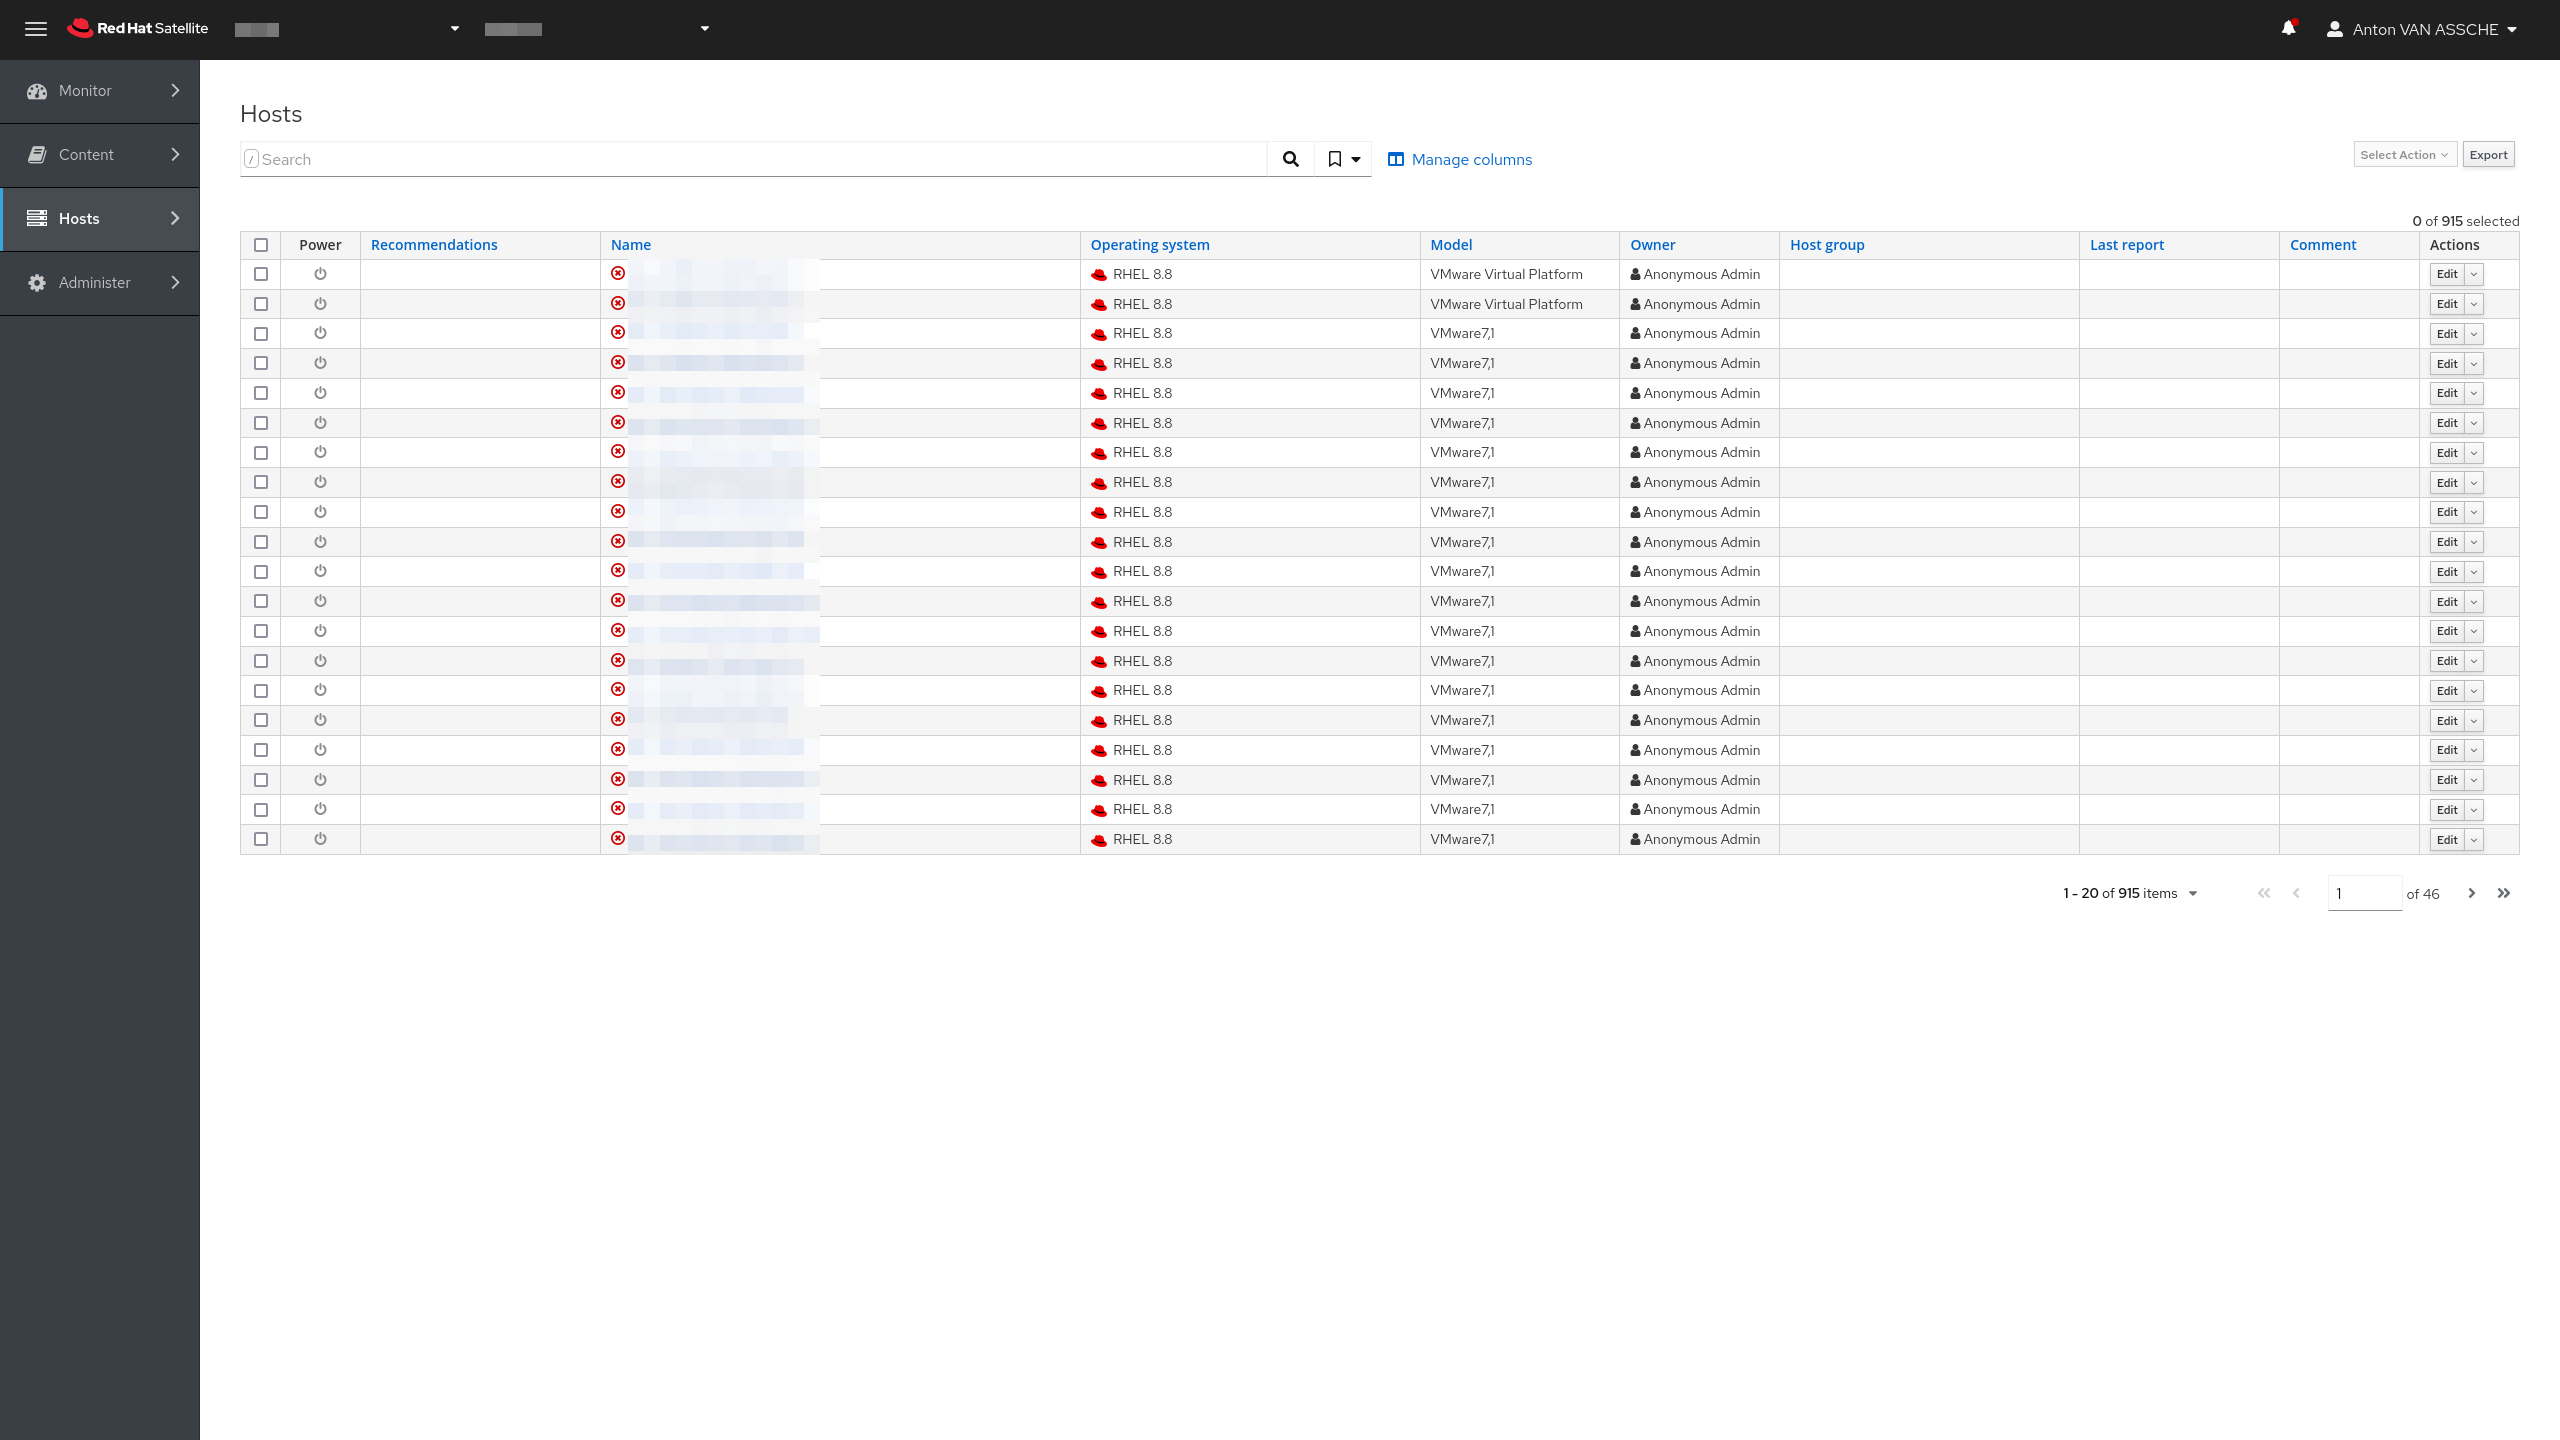
\includegraphics[width=\textwidth]
    {./graphics/state-of-the-art/rhel-satellite/rhel-sat-hosts.png}
    \caption[Hosts geregistreerd in Red Hat Satellite.]{\label{fig:rhel-sat-hosts}Lijst van hosts die geregistreerd zijn in Red Hat Satellite.}
\end{figure}

\begin{figure}[h!]
    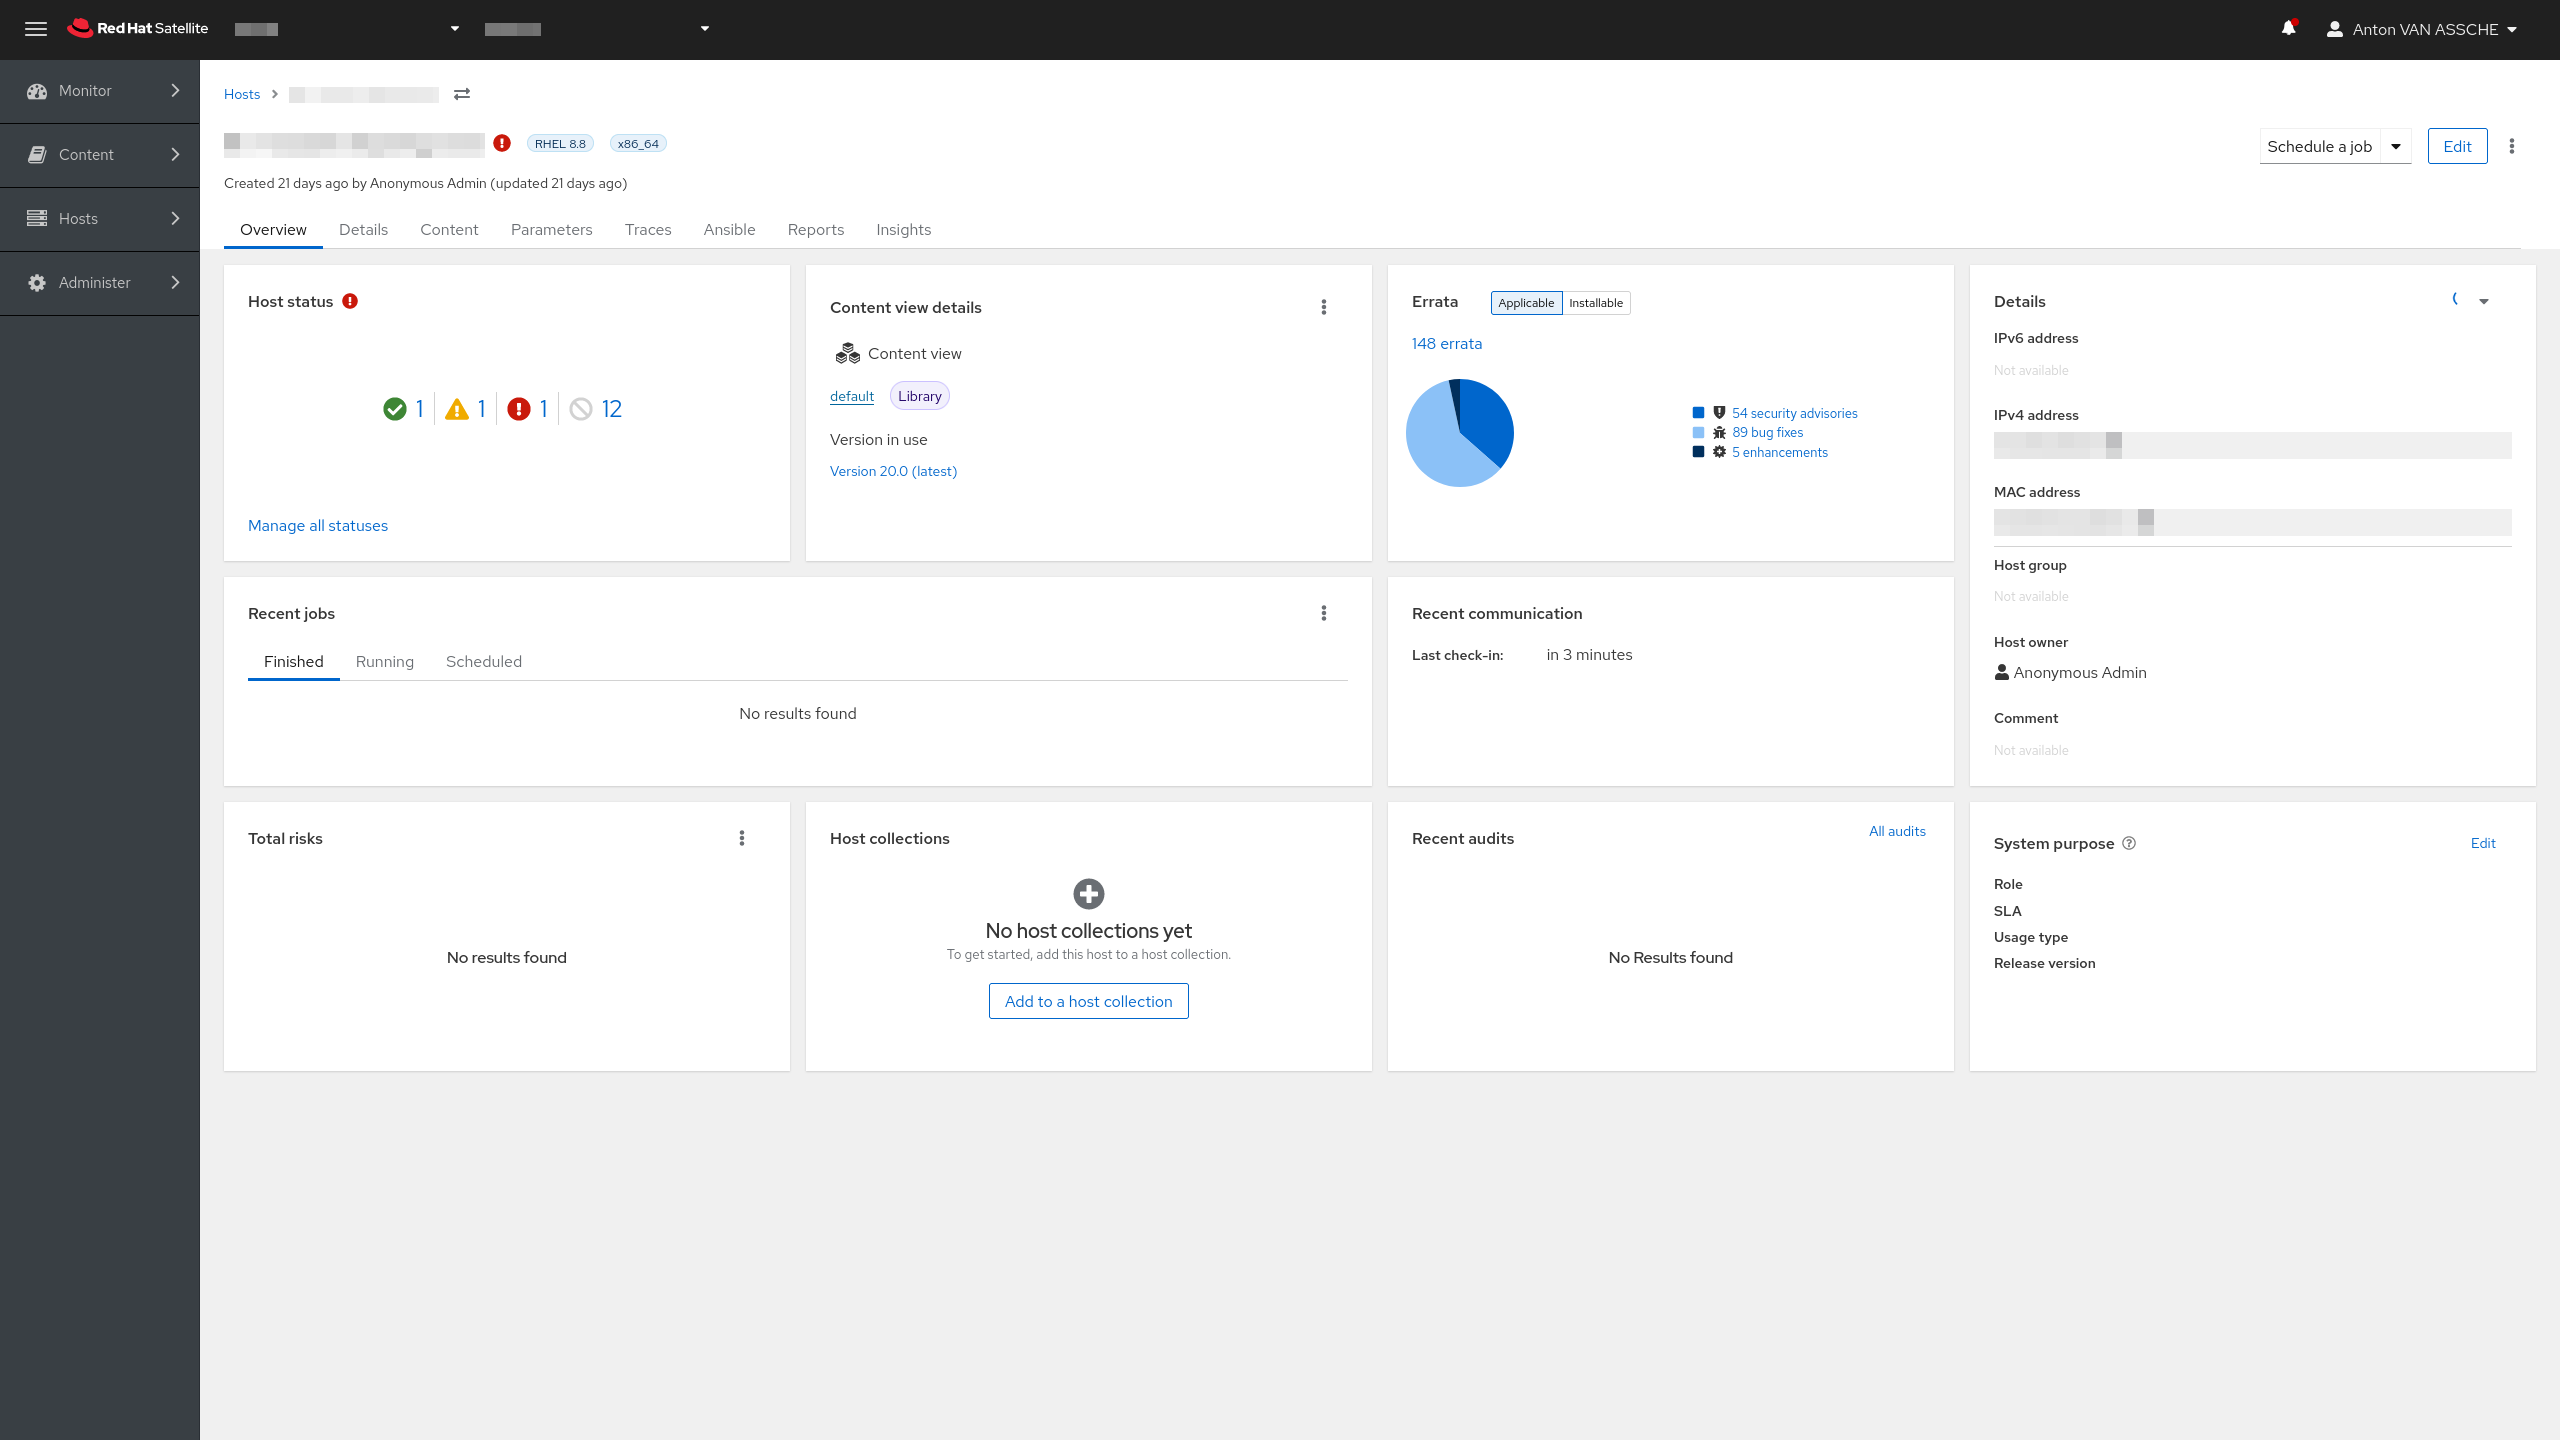
\includegraphics[width=\textwidth]
    {./graphics/state-of-the-art/rhel-satellite/rhel-sat-host-overview.png}
    \caption[Algemeen overzicht van host in Satellite.]{\label{fig:rhel-sat-host-overview}Algemeen overzicht van een host in Red Hat Satellite.}
\end{figure}

Door te navigeren naar het tabblad ``Details'' krijgen we een uitgebreider overzicht van de host te zien, zoals weergegeven in schermafbeelding~\ref{fig:rhel-sat-host-details}.
Hier worden veel meer gegevens over de host verstrekt, zoals het besturingssysteem, de kernelversie, de architectuur, informatie over geheugen en CPU en de netwerkinterfaces.
Vervolgens kunnen we doorklikken naar het tabblad ``Content'' en vervolgens naar ``Packages'', waar we een lijst krijgen van alle ge\"installeerde pakketten op de host, zoals weergegeven in schermafbeelding~\ref{fig:rhel-sat-host-pkgs}.
Klikken op een specifiek pakket geeft ons meer informatie over dat pakket, zoals de versie, de release, de grootte en de datum van installatie, deze informatie is echter niet zichtbaar in de schermafbeelding.

\begin{figure}[h!]
    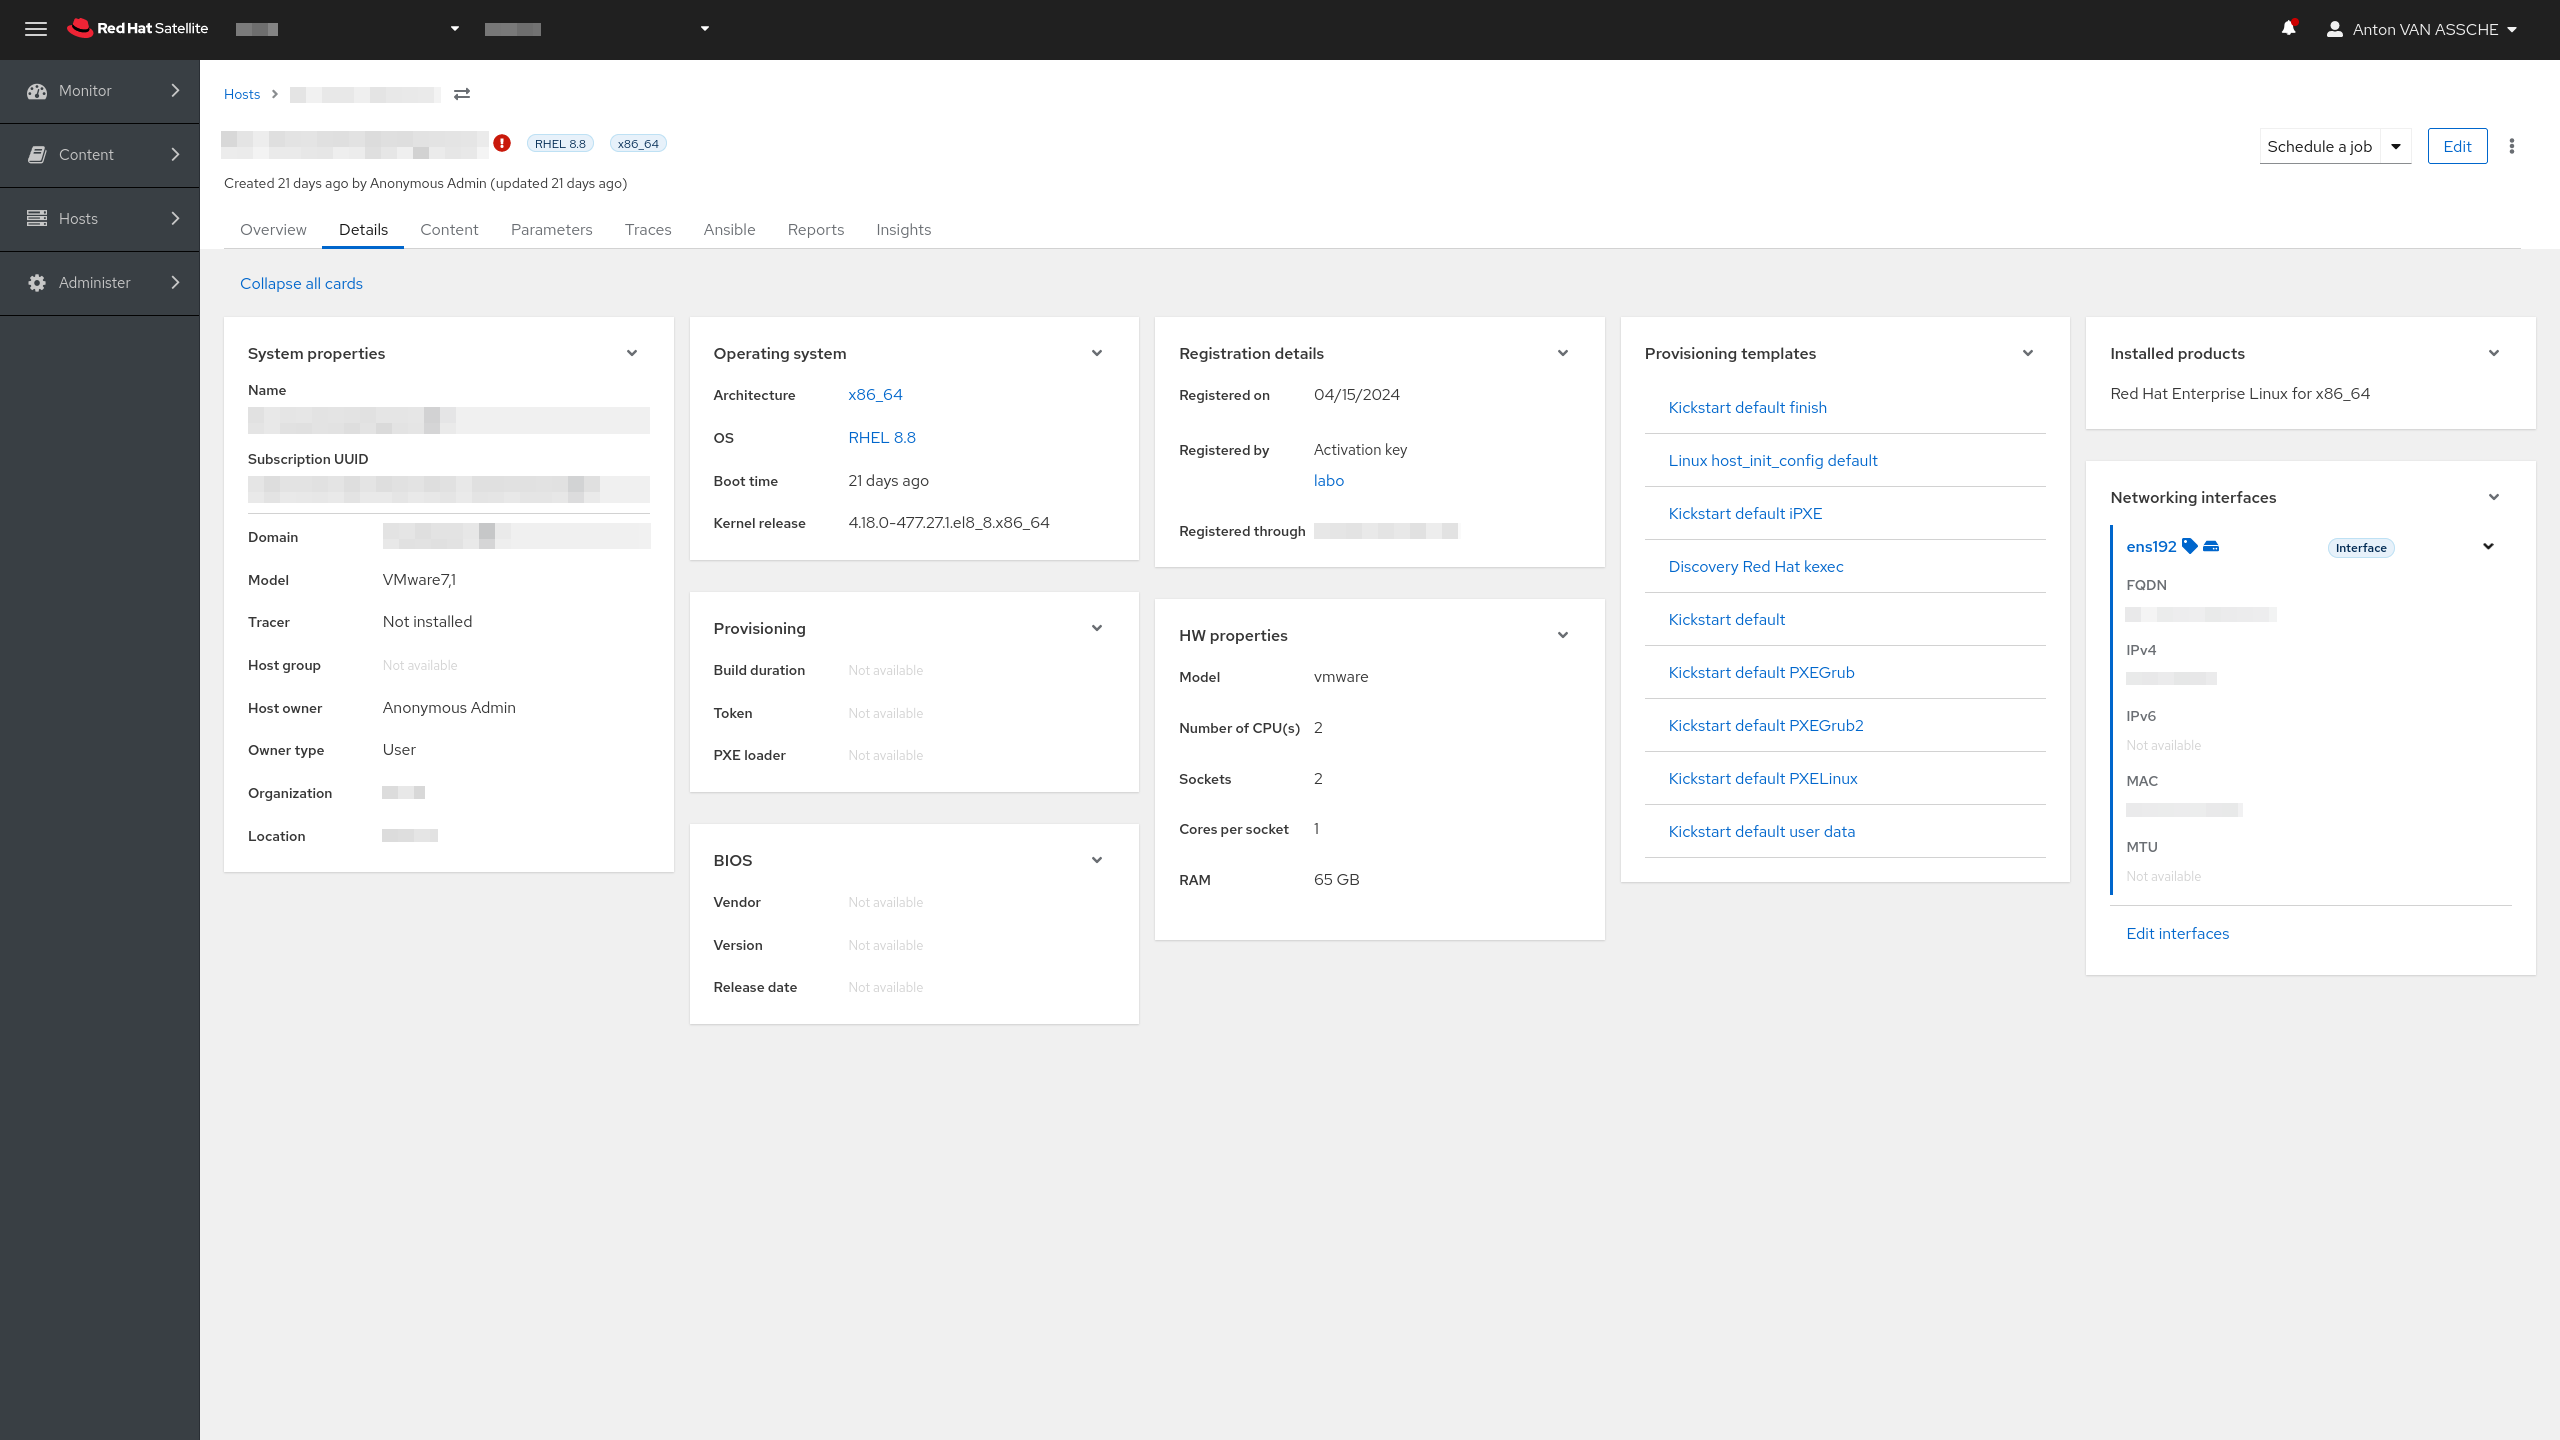
\includegraphics[width=\textwidth]
    {./graphics/state-of-the-art/rhel-satellite/rhel-sat-host-details.png}
    \caption[Details van host in Red Hat Satellite.]{\label{fig:rhel-sat-host-details}Details van een host in Red Hat Satellite.}
\end{figure}

\begin{figure}[h!]
    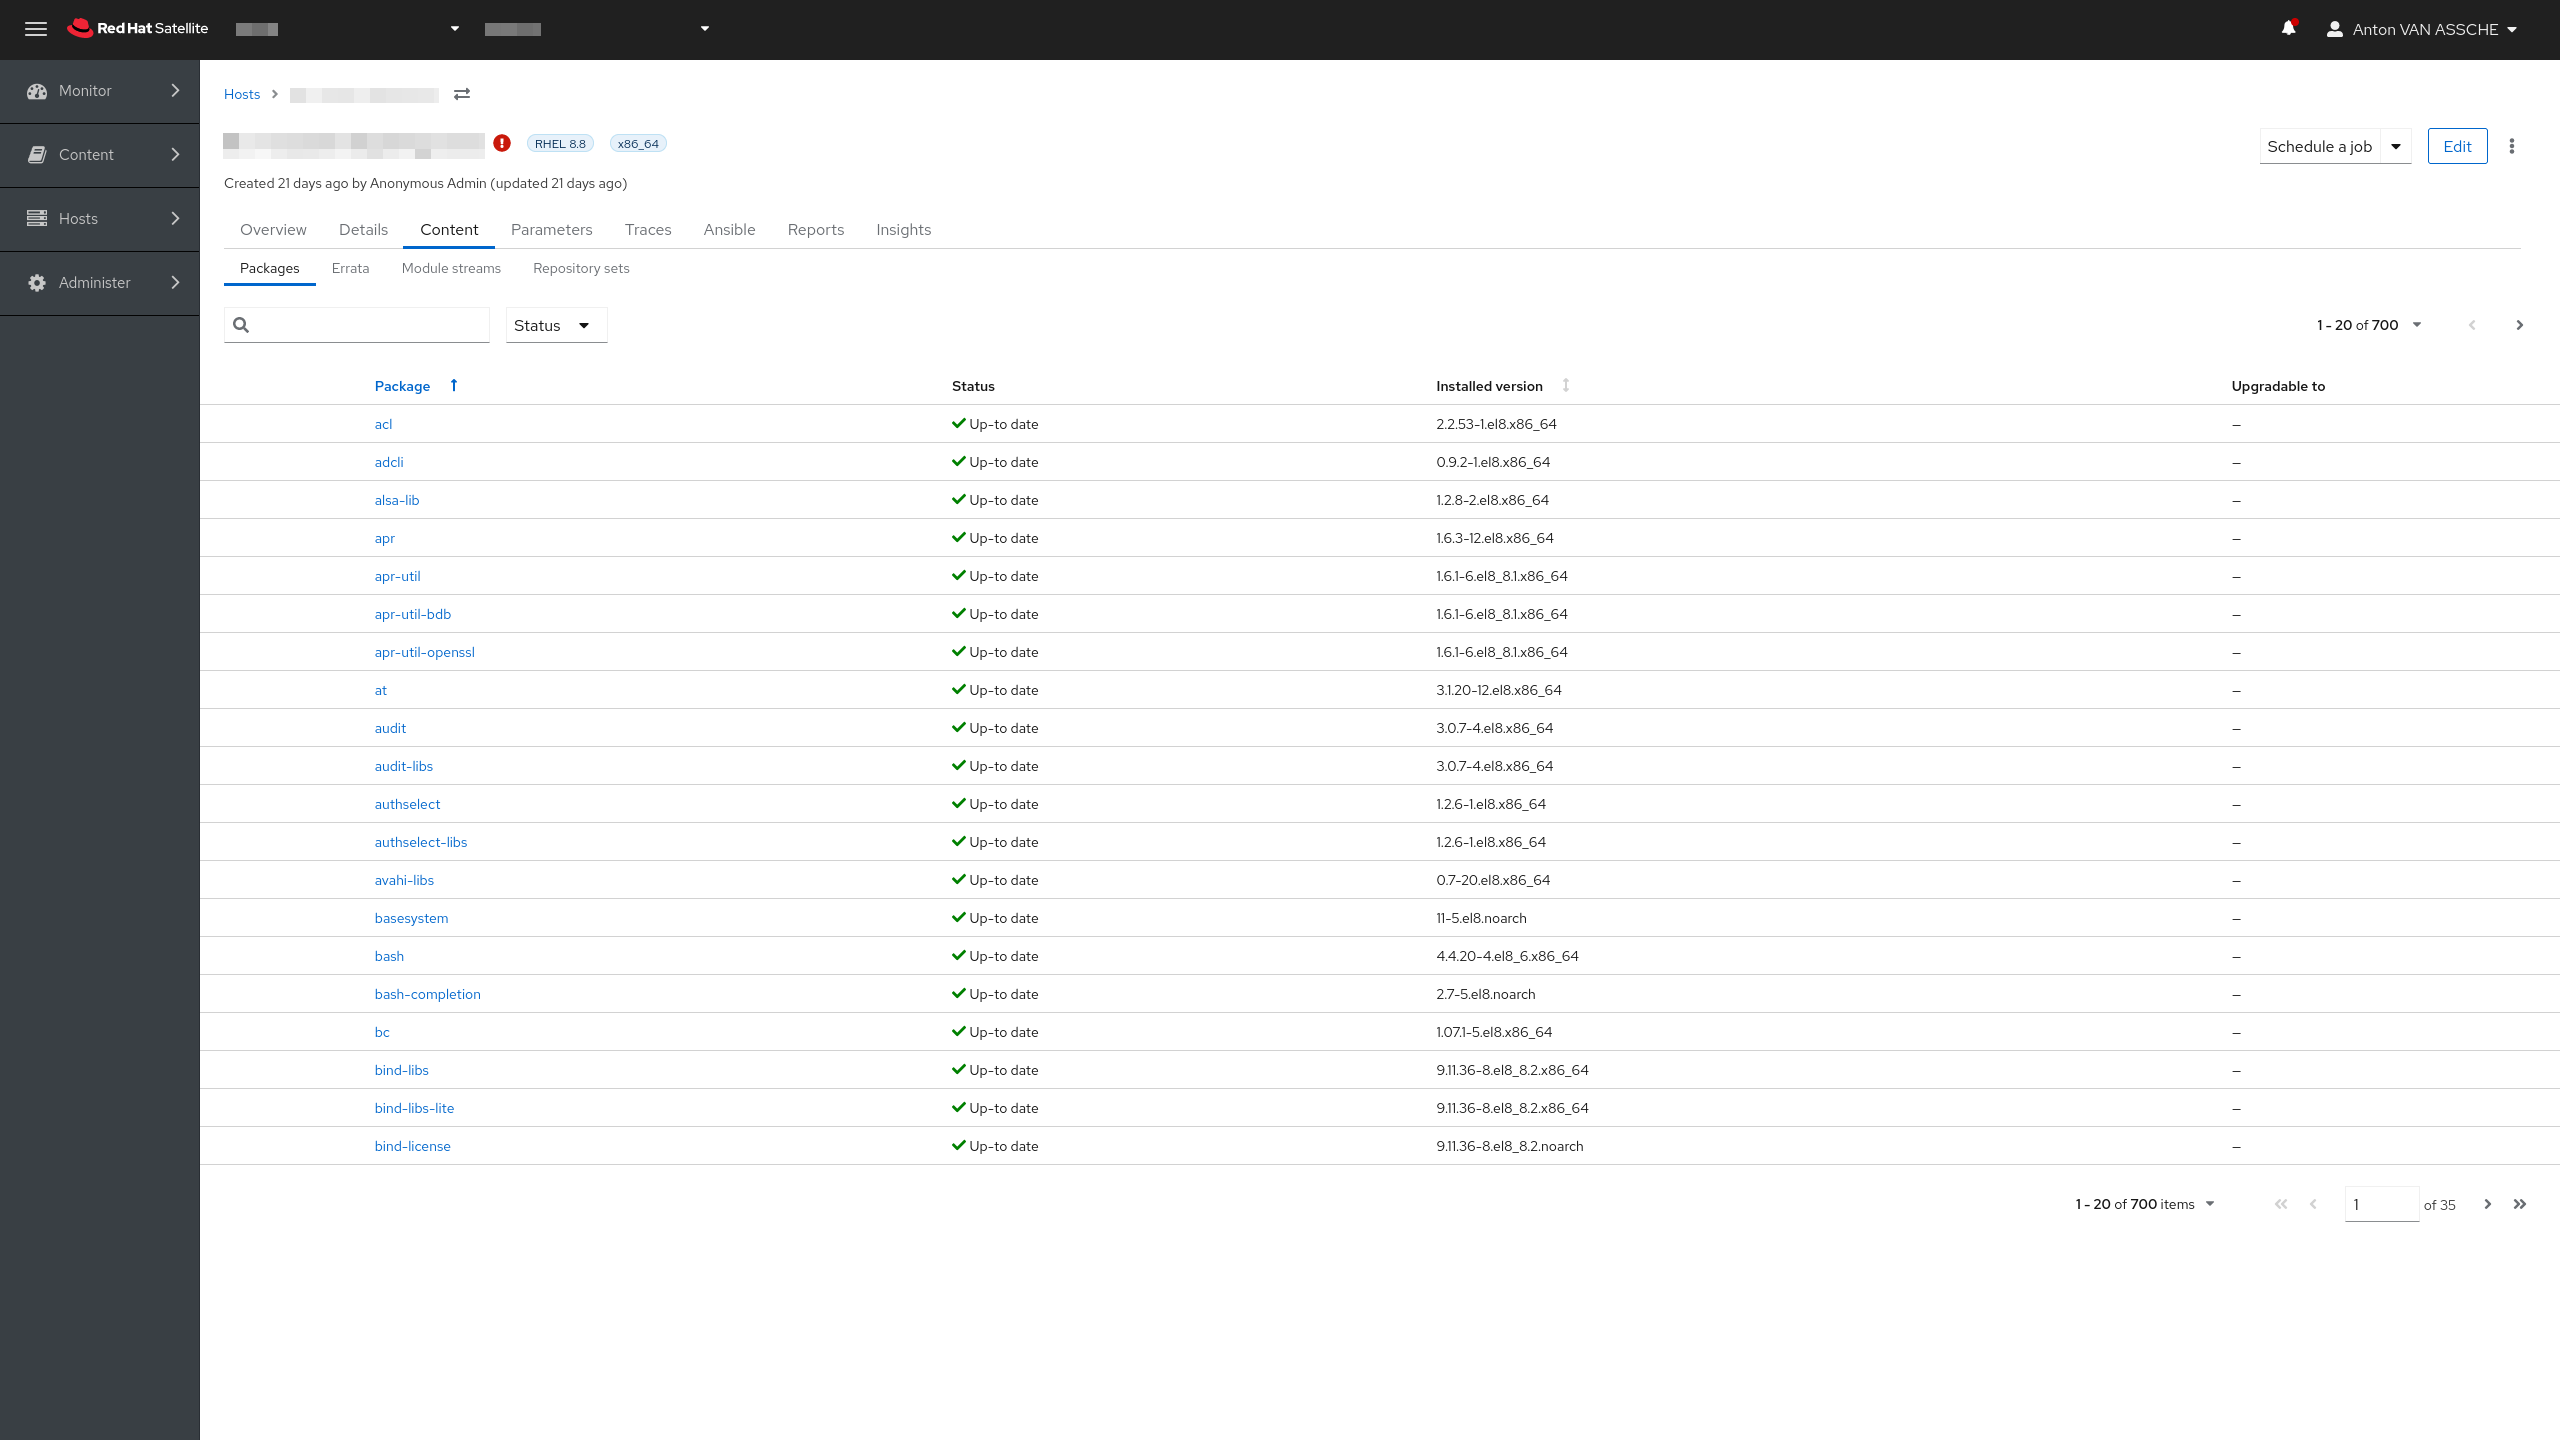
\includegraphics[width=\textwidth]
    {./graphics/state-of-the-art/rhel-satellite/rhel-sat-host-pkgs.png}
    \caption[Ge\"{i}nstalleerde packages op host in Satellite.]{\label{fig:rhel-sat-host-pkgs}Overzicht van ge\"{i}nstalleerde packages op een host in Red Hat Satellite.}
\end{figure}
